\documentclass[aspectratio=169,10pt]{beamer}
\usepackage[T1]{fontenc}
\usepackage{amsmath,amssymb,amsfonts}
\usepackage{bm}
\usepackage{tikz}
\usepackage{xcolor}
\usetikzlibrary{arrows.meta,positioning,shapes,calc}

\definecolor{parchment}{HTML}{F4E8C8}
\definecolor{paper}{HTML}{FAF1D8}
\definecolor{ink}{HTML}{1A1A1A}
\definecolor{inkgray}{HTML}{5A5A5A}
\definecolor{accentred}{HTML}{8B1A1A}
\definecolor{accentgreen}{HTML}{2D5F2C}
\definecolor{accentblue}{HTML}{1F4E79}
\definecolor{redbg}{HTML}{F7E0DE}
\definecolor{grnbg}{HTML}{E0EBDC}
\definecolor{blubg}{HTML}{DDE6EF}
\definecolor{labelbg}{HTML}{EFE0B0}

\usefonttheme{serif}
\setbeamercolor{background canvas}{bg=parchment}
\setbeamercolor{normal text}{fg=ink}
\setbeamercolor{structure}{fg=ink}
\setbeamercolor{frametitle}{fg=ink,bg=parchment}
\setbeamercolor{title}{fg=ink}
\setbeamercolor{itemize item}{fg=ink}
\setbeamercolor{itemize subitem}{fg=ink}
\setbeamercolor{item}{fg=ink}
\setbeamercolor{caption name}{fg=ink}
\setbeamertemplate{navigation symbols}{}
\setbeamertemplate{itemize item}{\textbullet}

\setbeamertemplate{frametitle}{%
  \vspace{0.30em}%
  \begin{center}%
    {\bfseries\Large\insertframetitle\par}%
    \vspace{0.28em}%
    {\color{ink}\rule{0.86\paperwidth}{0.4pt}}%
  \end{center}%
  \vspace{0.10em}%
}
\setbeamertemplate{footline}{%
  \hbox to \paperwidth{\hfil\itshape\small\insertframenumber\hspace{0.7em}}%
  \vspace{0.35em}%
}

\newcommand{\vY}{\bm{Y}}
\newcommand{\vy}{\bm{y}}
\newcommand{\vA}{\bm{A}}
\newcommand{\vB}{\bm{B}}
\newcommand{\valpha}{\bm{\alpha}}
\newcommand{\vn}{\bm{n}}
\newcommand{\vs}{\bm{s}}
\newcommand{\vW}{\bm{W}}
\newcommand{\T}{^{\mathsf T}}
\newcommand{\Hh}{^{\mathsf H}}
\newcommand{\norm}[1]{\left\lVert #1\right\rVert}
\DeclareMathOperator*{\argmin}{arg\,min}

\tikzset{
  flowbox/.style={draw=ink,fill=paper,line width=0.6pt,
                  minimum width=2.5cm,minimum height=1.0cm,
                  align=center,font=\small\bfseries,inner sep=4pt},
  smallbox/.style={draw=ink,fill=paper,line width=0.4pt,
                   minimum width=0.7cm,minimum height=0.55cm,
                   inner sep=2pt,align=center,font=\footnotesize\itshape},
  method/.style={draw=accentgreen,fill=grnbg,line width=1.0pt,
                 align=center,font=\small\bfseries,inner sep=6pt},
  issue/.style={draw=accentred,fill=redbg,line width=1.0pt,
                align=center,font=\small\bfseries,inner sep=6pt},
  idea/.style={draw=accentblue,fill=blubg,line width=1.0pt,
               align=center,font=\small\bfseries,inner sep=6pt},
  flowarr/.style={-{Stealth[length=2.5mm,width=2mm]},line width=0.7pt},
  softarr/.style={-{Stealth[length=2mm,width=1.6mm]},line width=0.5pt,color=inkgray}
}

\newcommand{\bottomnote}[1]{%
  \begin{center}{\itshape\small #1}\end{center}}

\newcommand{\papercover}[4]{%
  \begin{frame}[plain]
    \vfill
    \begin{center}
      {\bfseries\Huge #1\par}
      \vspace{0.8cm}
      {\Large #2\par}
      \vspace{0.35cm}
      {\itshape\large\color{inkgray}#3\par}
      \vspace{0.55cm}
      {\small\texttt{\detokenize{#4}}\par}
    \end{center}
    \vfill
  \end{frame}}

\newcommand{\twocolmodel}[4]{%
  \begin{columns}[T,onlytextwidth]
    \begin{column}{0.48\textwidth}#1\end{column}
    \begin{column}{0.48\textwidth}#2\end{column}
  \end{columns}
  \bottomnote{#3\\#4}}


\begin{document}

\papercover
  {Progressive ICI Equalization}
  {Jianzhong Huang, Zhou, Jie Huang, Berger, and Willett}
  {IEEE Journal of Selected Topics in Signal Processing, 2011}
  {progressive_ici_equalization_ofdm_uwa.pdf}

\begin{frame}{1. Core problem}
\twocolmodel{
  \begin{itemize}\setlength{\itemsep}{0.45em}
    \item Mild channels decode with a narrow ICI model
    \item Severe Doppler spread needs a wider span
    \item A fixed worst-case receiver wastes effort
  \end{itemize}
}{
  \[
    Y_k
    =
    \sum_{q=k-B}^{k+B}
    H_{kq}X_q+n_k
  \]
  \[
    B \;\text{small first, larger only if needed}
  \]
}{
  The receiver adapts the model complexity during decoding.
}{
  While a fixed worst-case span is simple, it spends complexity that easy conditions do not require.
}
\end{frame}

\begin{frame}{2. Progressive loop}
\begin{center}
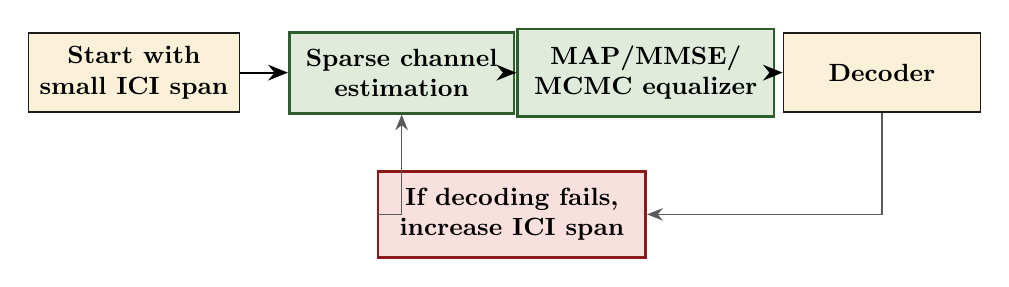
\begin{tikzpicture}[x=1cm,y=1cm]
  \node[flowbox] (small) at (-4.8,0.7) {Start with\\small ICI span};
  \node[method,minimum width=2.8cm] (est) at (-1.4,0.7) {Sparse channel\\estimation};
  \node[method,minimum width=2.6cm] (eq) at (1.7,0.7) {MAP/MMSE/\\MCMC equalizer};
  \node[flowbox] (dec) at (4.7,0.7) {Decoder};
  \node[issue,minimum width=3.4cm] (grow) at (0,-1.1) {If decoding fails,\\increase ICI span};
  \draw[flowarr] (small) -- (est);
  \draw[flowarr] (est) -- (eq);
  \draw[flowarr] (eq) -- (dec);
  \draw[softarr] (dec.south) |- (grow.east);
  \draw[softarr] (grow.west) -| (est.south);
\end{tikzpicture}
\end{center}
\bottomnote{Complexity is spent only after the decoder reports that the current model is insufficient.}
\end{frame}

\begin{frame}{3. Algorithm skeleton}
\begin{enumerate}\setlength{\itemsep}{0.45em}
  \item Narrow ICI band, pilot-aided sparse channel estimate
  \item Equalize by a soft-input method; pass LLRs to the decoder
  \item Stop if the decoder succeeds
  \item Otherwise enlarge the span, reuse decoder soft information
  \item Repeat until success or maximum span
\end{enumerate}
\bottomnote{The ICI span is a working hypothesis driven by decoder feedback, not a fixed assumption.}
\end{frame}

\begin{frame}{4. JUNA connection}
\begin{itemize}\setlength{\itemsep}{0.5em}
  \item Progressive ICI half-width as a discrete model-selection variable
  \item Start cheap:
  \[
    \mathcal B_1(k)\subset\mathcal B_2(k)\subset\cdots
  \]
  and expand only when residual energy or parity checks demand it.
  \item Decoder soft information feeds back into channel estimation
  \item Inference improves by changing the model during iterations
\end{itemize}
\bottomnote{This paper and JUNA share one premise: the model may change while decoding.}
\end{frame}

\end{document}
